\section{Art Style}
The art style of \ourgame{} is largely influenced by the individual styles and previous works of \ourteam{}'s art department.

\begin{figure}[H]
\centering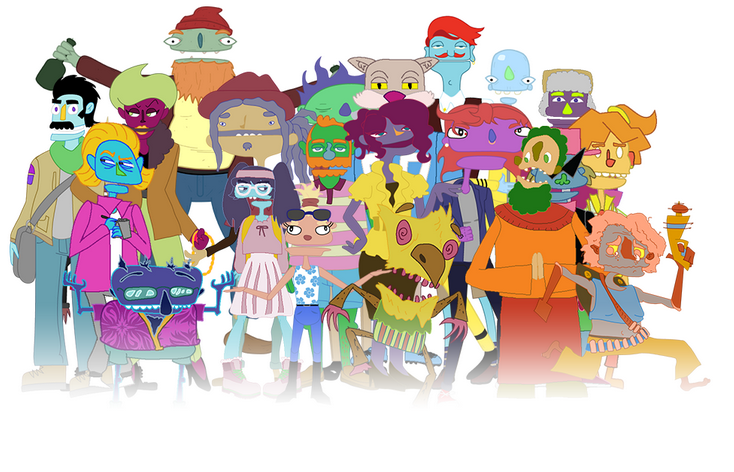
\includegraphics[width=0.7\linewidth]{images/art_style}
\end{figure}

\clearpage
Ian's characters, shown in Figure~\ref{fig:i1}, were a starting point from which \ourgame{}'s character designs stemmed from. \ourgame{}'s character's concepts were also inspired by Michael's art for a previous game, \textit{"This Is Our Game And I'm Out Of Ideas"}, seen in Figure~\ref{fig:m3}, where characters were broken into components and moved strangely, possessing inhuman freedom in joint movement. 
The base structure for the characters can be described as bipedal humanoids. While many of the characters are humans, there are also a variety of mythological creatures and mechanical beings included. Anthropomorphic and folklore themes were explored and incorporated into some of the character designs, presented as mundane beings sporting modern clothing. The mixture of human and non-human characters creates a more surreal style. 
Tall characters tend to be more lanky and creepy, with irregular human body proportions emphasizing long and thin limbs. These can be seen in the original concept art in Figure\ref{fig:m4}. Similarly, short characters have more blocked out and stubby limbs. This gives them a more grounded appearance. Some of the human characters sport distinctive clothing based off modern subcultures to exaggerate their personalities. Details in apparel and fashion statements gives the characters more distinctive features.



\begin{figure}[H]
\begin{subfigure}{.4\textwidth}
    \centering
    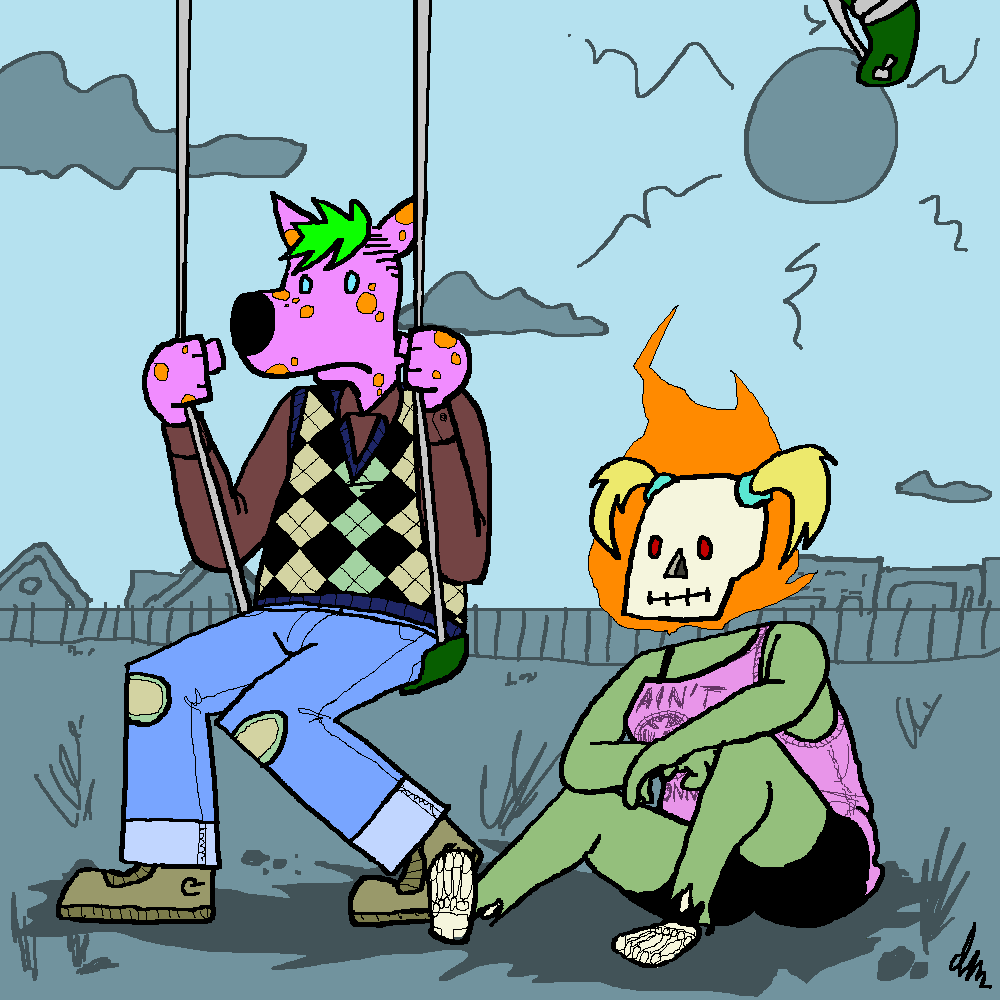
\includegraphics[width=.9\linewidth]{images/ref_IAN01}
  	\caption{Comic - \textit{Monster Friends in "Halloween"}}
  \label{fig:i1}
  \end{subfigure}
  \begin{subfigure}{.5\textwidth}
    \centering
    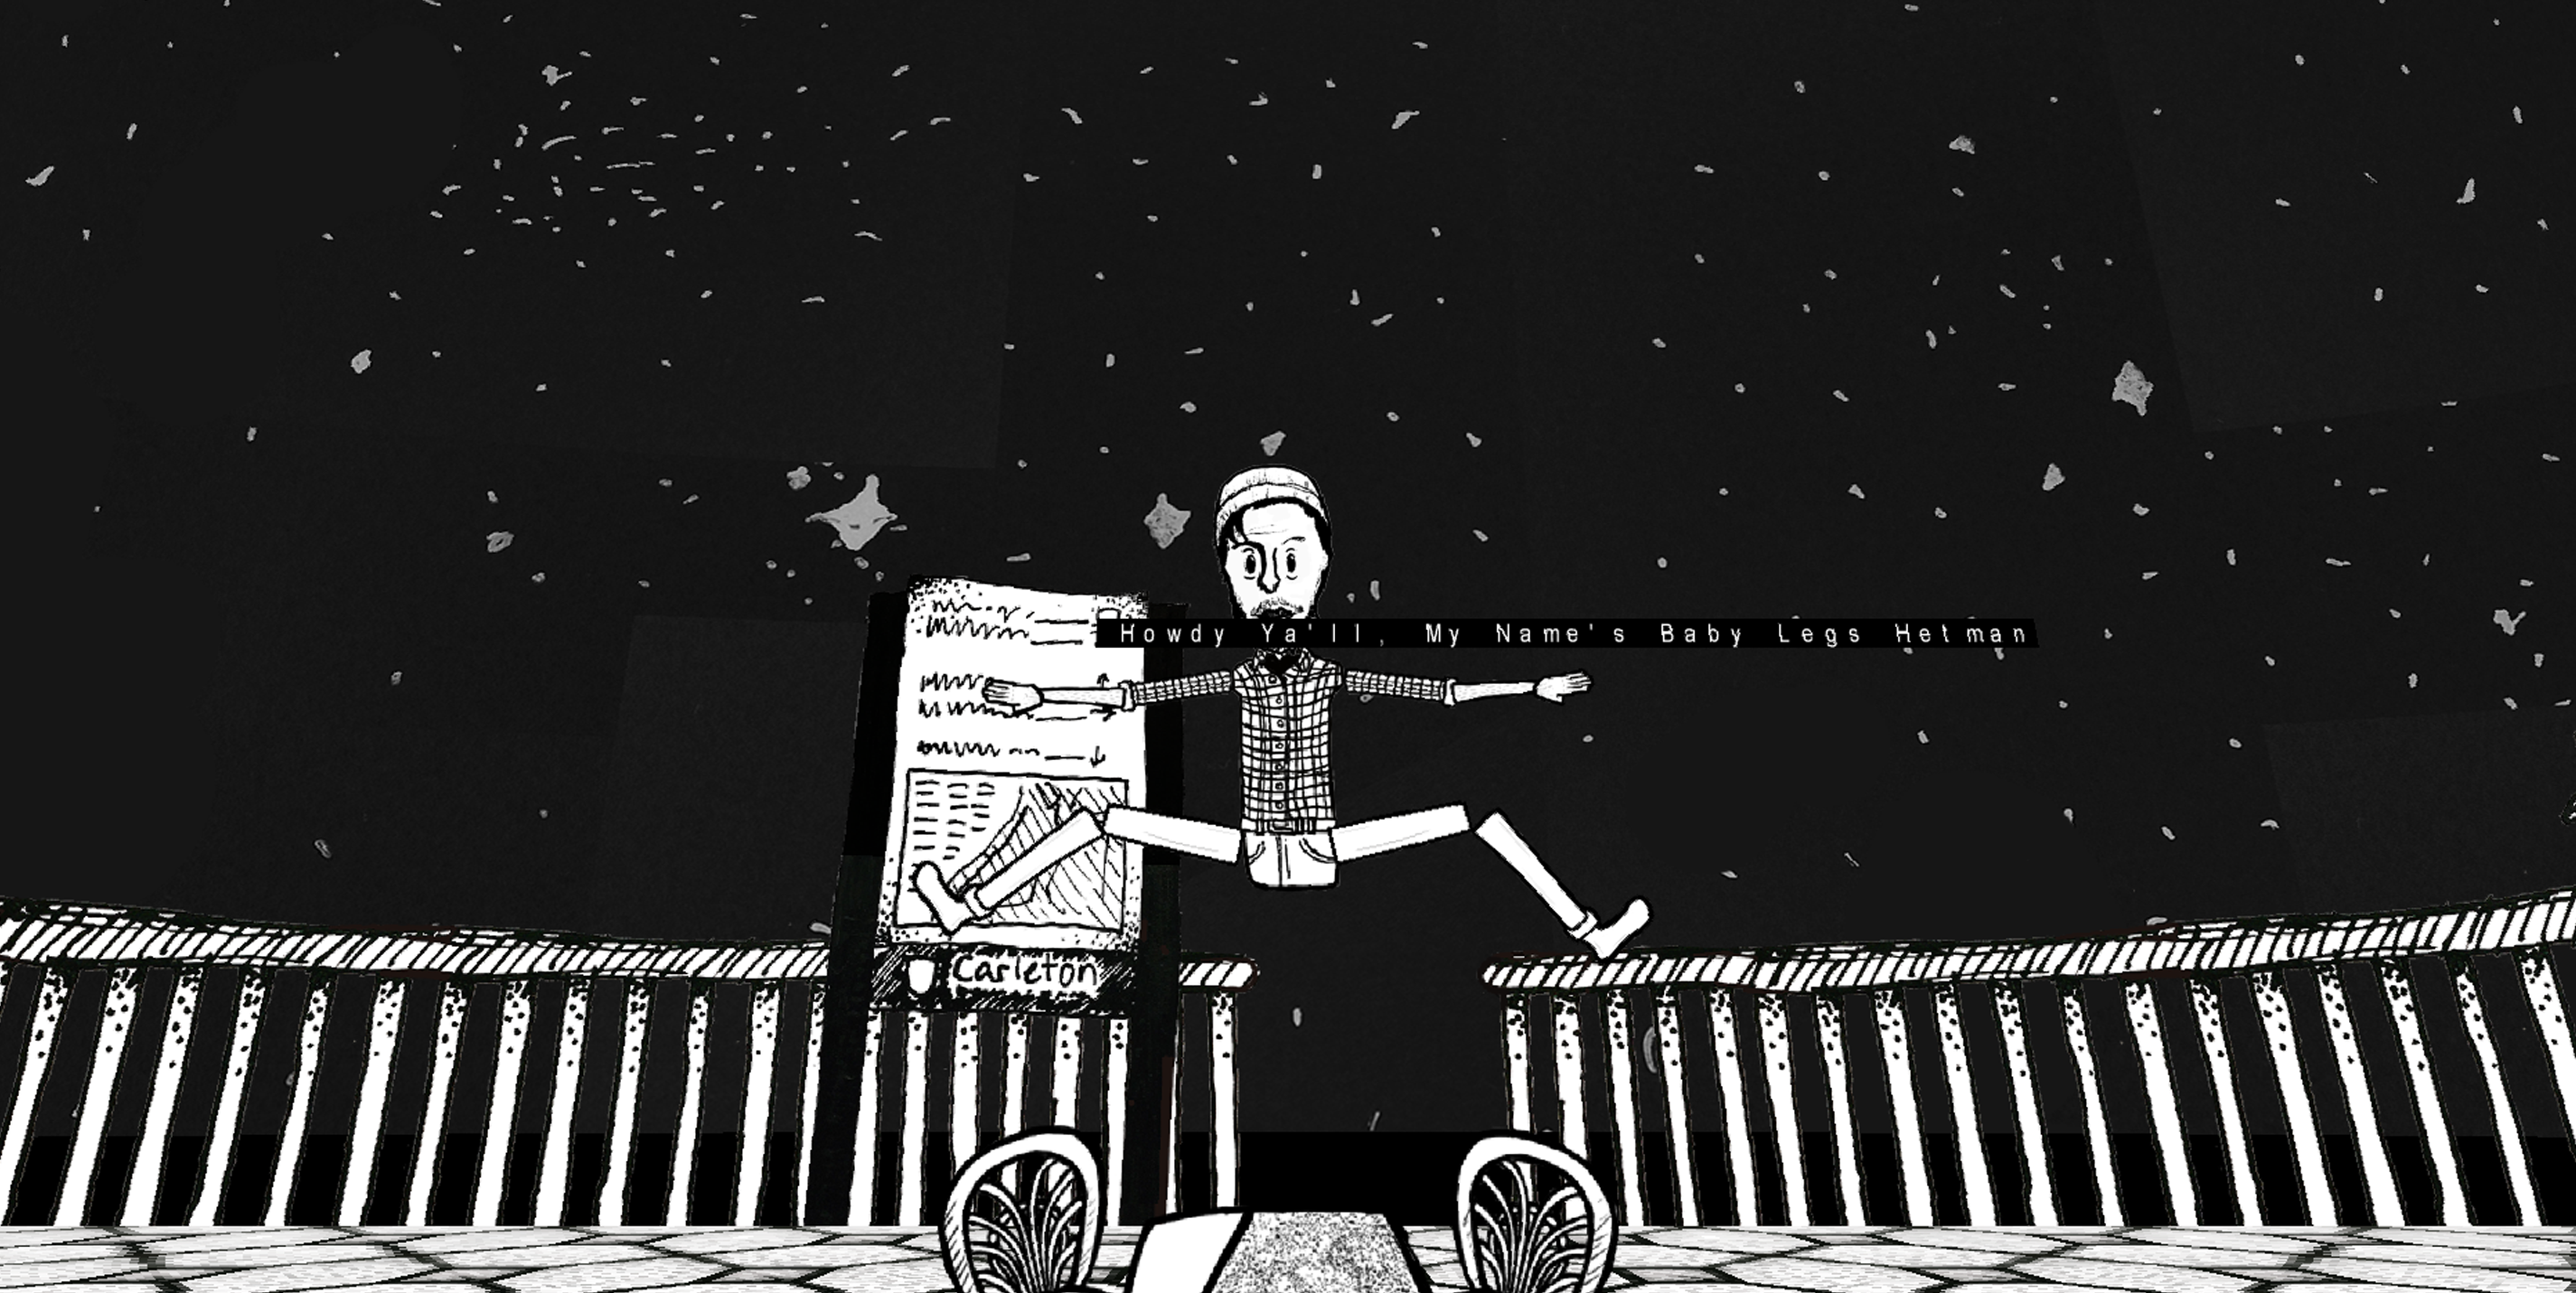
\includegraphics[width=.9\linewidth]{images/ref_MICHAEL03}
    \caption{Character in TIOGAIOOI}
    \label{fig:m3}
  \end{subfigure}
  \begin{subfigure}{.45\textwidth}
    \centering
    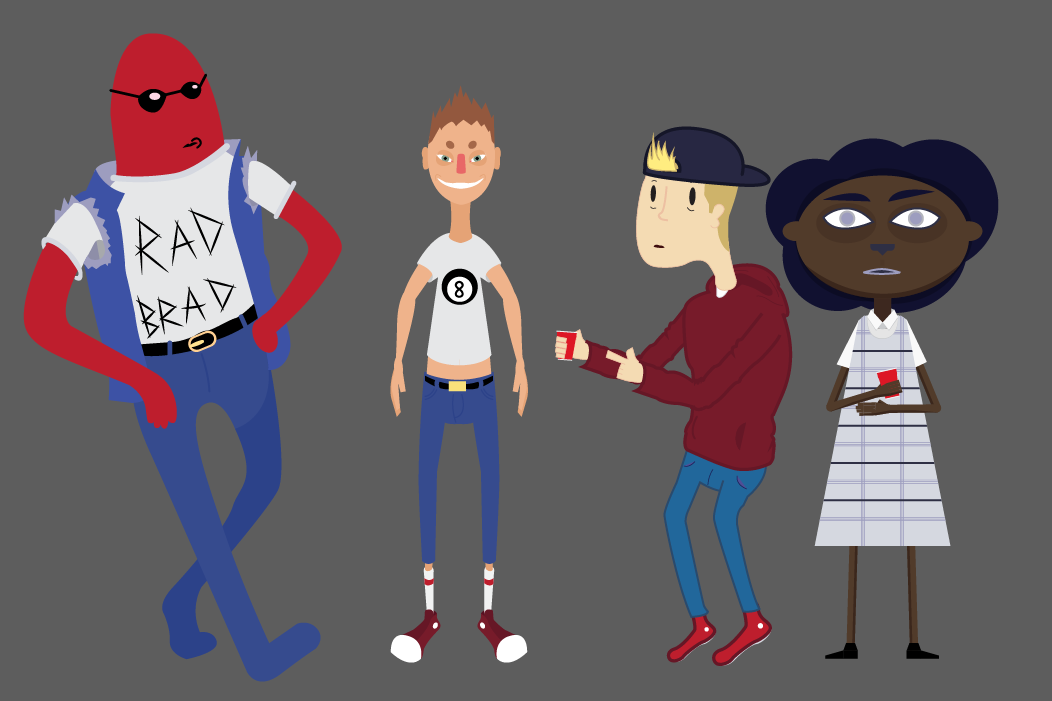
\includegraphics[width=.9\linewidth]{images/ref_MICHAEL04}
    \caption{Initial Character Ideas}
    \label{fig:m4}
  \end{subfigure}
  \caption{Michael's Art Style}
  \label{fig:mstyle}
\end{figure}
